% !TeX root = ../../../../../../thesis.tex


%Both figure side by side to save space...
	%\begin{figure}[!tbp]
	%  \centering
	%  \begin{minipage}[b]{0.48\textwidth}
	%    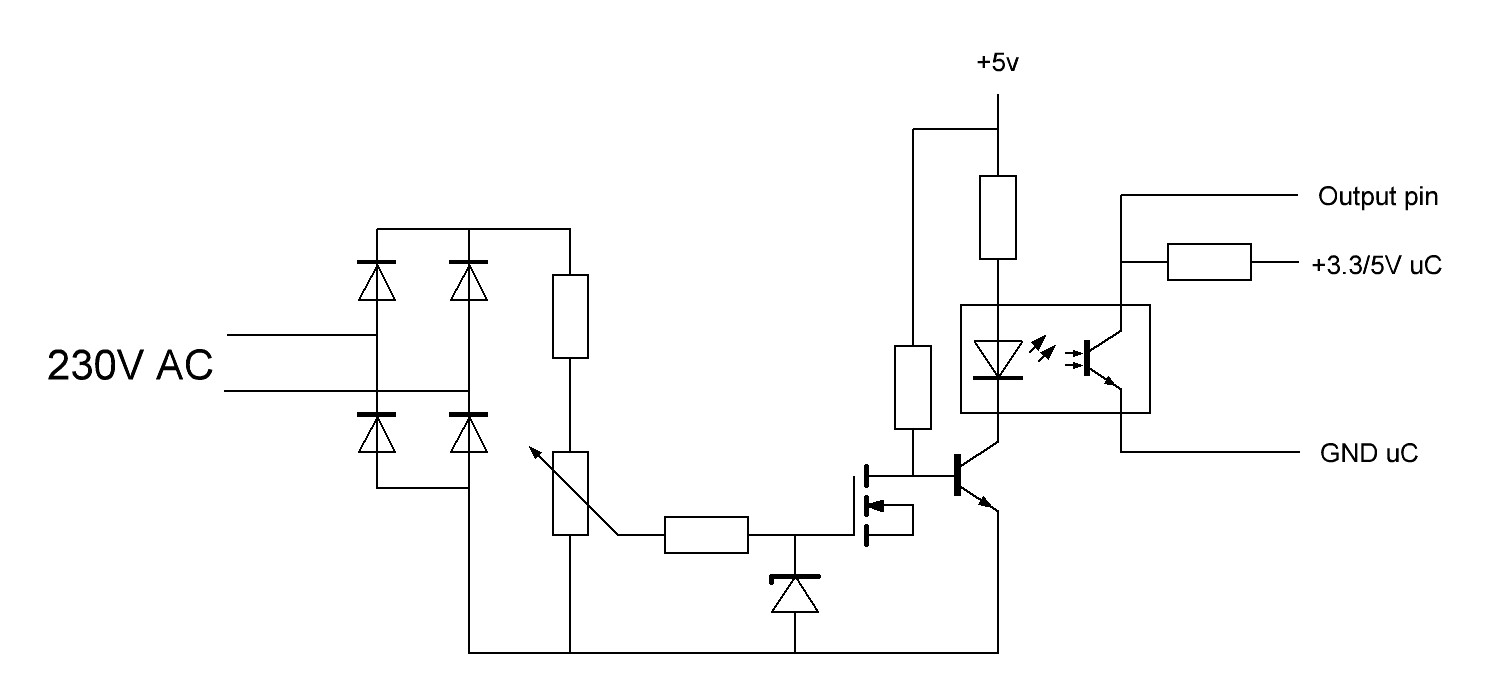
\includegraphics[width=\textwidth]{chapters/hardware-chapters/custom-modulator-trigger.JPG}
	%    \caption{Triggering circuit to determine when the voltage is sufficiently high enough to start encoding information.}
	%	\label{fig:custom-modulator-trigger}
	%  \end{minipage}
	%  \hfill
	%  \begin{minipage}[b]{0.48\textwidth}
	%    \includegraphics[width=\textwidth]{chapters/hardware-chapters/custom-modulator-voltage-source.JPG}
	%    \caption{Non-disturbing voltage source to power other parts of the circuit.}
	%	\label{fig:custom-modulator-voltage-source}
	%  \end{minipage}
	%\end{figure}



\subparagraph{Non-disturbing Voltage Source}

		
	The two parts of the custom modulator which solve the translation problem of mapping zeros and ones of the ID into the current draw, have now been explained in the prior sections: The triggering circuit and the current source implementation.
	However, as can be seen from the schematics of these parts (\autoref{fig:triggering-circuit-output-2} and \autoref{fig:custom-modulator-current-source}), a 5 Volt voltage source is required to power parts of these circuits.
	In this section it will be explained where this voltage comes from and how it is able to provide this voltage while not distorting the distinct current signature of the ID.


	In the triggering circuit section, it is explained that the LEDs need 100 V before they draw current.
	So every time the voltage is above 100 V the encoding of the ID may begin and whenever the voltage drops below 100 V the encoding stops.
	So whenever the voltage is below 100 V, it does not matter what current is drawn, because no encoding of the ID will take place there.
	Below 100 V is an ideal place to let a circuit create a stable 5 V output to power the triggering circuit and the current source, because it will not distort the encoding of the ID.

	As mentioned before the time that is available for modulation, is 16 ms per period of 20 ms.
	During 16 ms, the voltage is above 100 V and $20 - 16 = 4$ ms is the time that the voltage is below 100 V.
	So in 4 ms per period of 20 ms, it is allowed to draw any current necessary to store the required energy to power the trigger and current source circuits.
	And in the remaining 16 ms per period of 20 ms, this stored energy will be consumed by the triggering circuit and the current source.
	During this 16 ms no current will be drawn to create the stable 5 V output.% as this is already done in the 4 ms window when the voltage is below 100 V.

	To store the energy that will be used later on, a capacitor is used.
	The output of this capacitor goes to a voltage stabilizer IC that will ensure a stable 5 V output.
	A schematic of the solution can be found in \autoref{fig:custom-modulator-voltage-source}.
	When the capacitor is empty, the capacitor is charged by the AC only when the voltage is below 100 V.
	The charging of the capacitor causes a current spike as could already be seen in \autoref{fig:current-source-measurement-annotated}.
	In this figure, regions C1 and C2 clearly show this current spike.
	But since no encoding is done in this region, it will not interfere with the encoding.
	This solution provides a continuous stable 5 V voltage source without distorting the encoding of the ID, since the encoding and the voltage source work in different time sections.

	\begin{figure}[t]
		\centering
		\includegraphics[angle=0,width=0.8\textwidth]{chapters/hardware-chapters/AC/ac-modulator/custom-hardware/ac-voltage-source/custom-modulator-voltage-source.JPG}
		\caption{Non-disturbing voltage source to power other parts of the circuit.}
		\label{fig:custom-modulator-voltage-source}
	\end{figure}
	
